For our experiment, we set up our Pi in Alden Hall.  It was placed near the doors to room 101 and faced down the hallway between 6:00PM and 7:00PM.  During this time period, the Pi detected a person and uploaded a picture to dropbox a total of 18 times.  Considering the time for which it was set up, we believe this is a resonable number of detections over an hour.  Of the 18 detections, all subjects were correctly identified 13 times.  In 3 detections, only some of the subjects were properly detected (e.g. only found one person when two are present), or it correctly identified all subjects and more (e.g. found three people when two are present).  In the remaining 2, the program failed to properly draw a bounding box over any of the subjects.  With these 2 failures, though, they seem to be due to how close the subjects were to the camera --- the subjects either weren't fully visible in the frame, or they took up a large portion of the frame.

\begin{figure}[h]
\centering
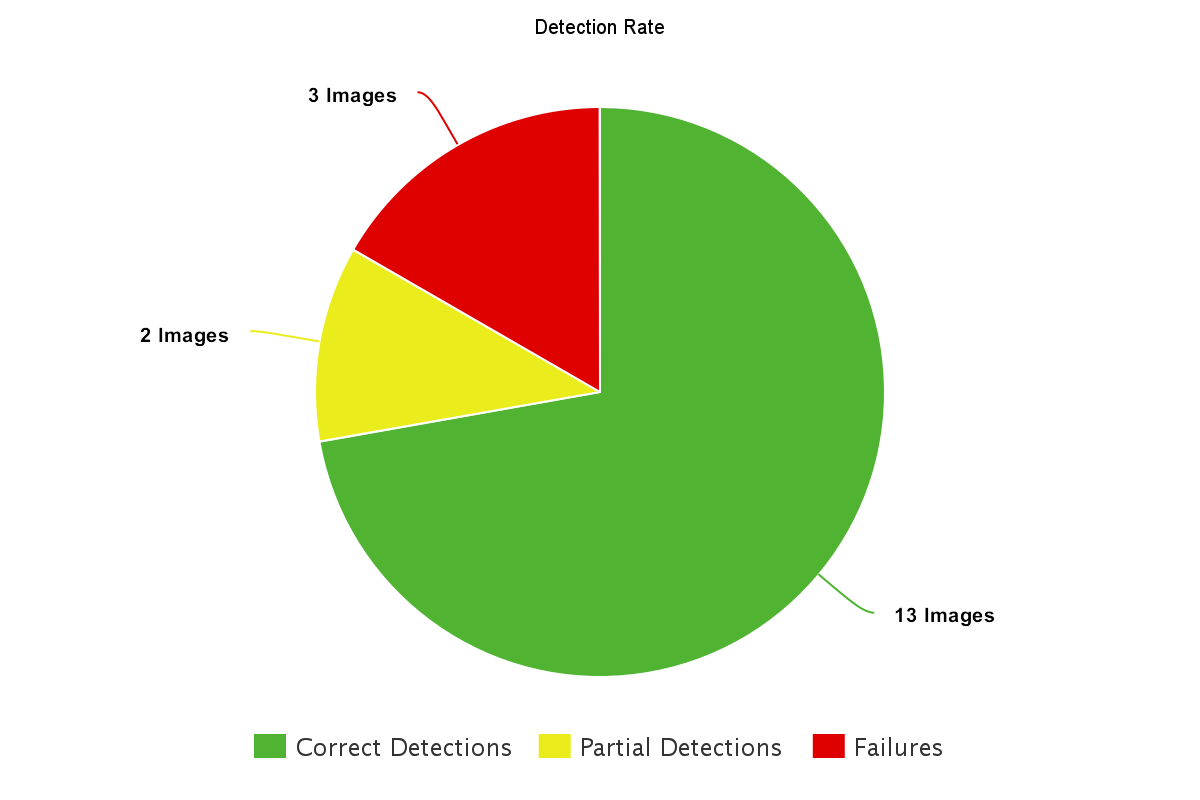
\includegraphics[scale=.25]{images/DetectionRate.png}
\end{figure}

\begin{figure}[h]
\minipage{0.32\textwidth}
  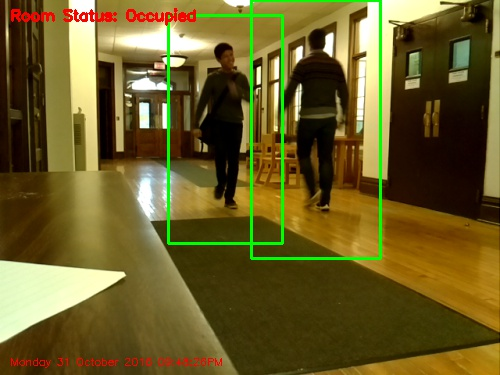
\includegraphics[width=\linewidth]{images/body1.jpg}
  %\caption{A really Awesome Image}\label{fig:awesome_image1}
\endminipage\hfill
\minipage{0.32\textwidth}
  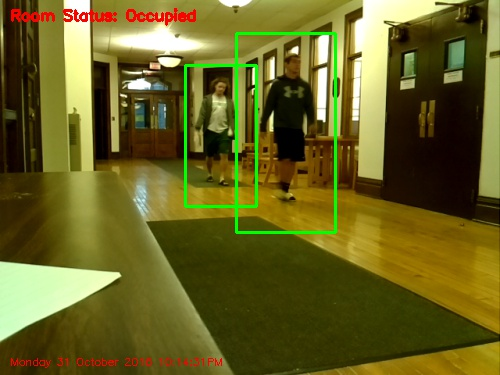
\includegraphics[width=\linewidth]{images/body2.jpg}
  %\caption{A really Awesome Image}\label{fig:awesome_image2}
\endminipage\hfill
\minipage{0.32\textwidth}%
  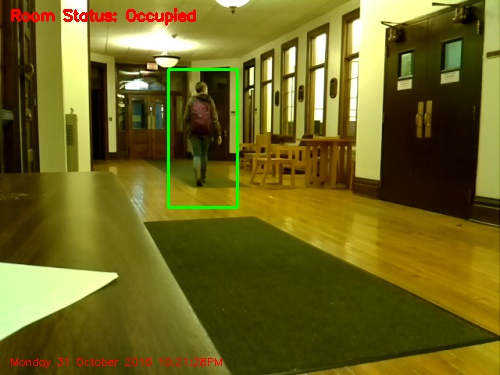
\includegraphics[width=\linewidth]{images/body3.jpg}
  %\caption{A really Awesome Image}\label{fig:awesome_image3}
\endminipage
\caption{Three Examples of Successful Detection}
\end{figure}


\begin{figure}[h]
        \centering
        \begin{subfigure}[b]{0.45\textwidth}
                \centering
                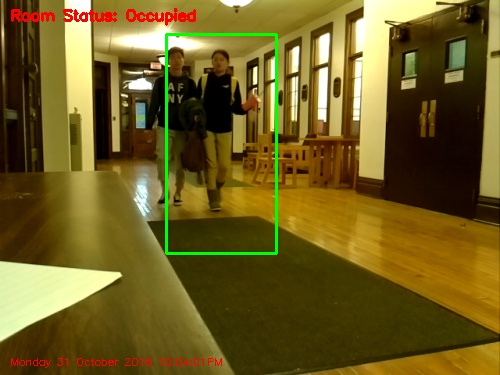
\includegraphics[width=\textwidth]{images/body4.jpg}
                \caption{Partial Detection}
                \label{fig:sensor3}
        \end{subfigure}%    <-- % added here
        \hfill %% useful if width of each figure is less the .5\textwidth
        \begin{subfigure}[b]{0.45\textwidth}
                \centering
                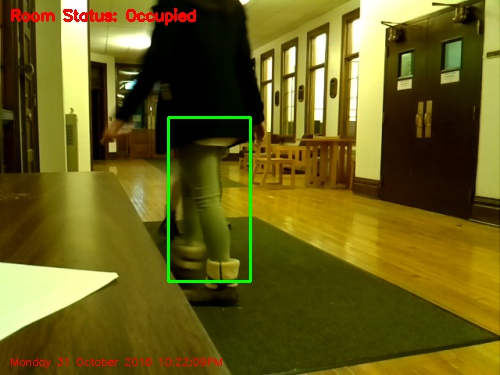
\includegraphics[width=\textwidth]{images/body5.jpg}
                \caption{Failed Detection}
                \label{fig:tiger}
        \end{subfigure}
        \caption{Partial and Failed Detection}
\end{figure}

\pagebreak